We have established that small HD explains the remarkable performance of HL.
In the same spirit, we introduce a notion that allows for the construction of provably efficient HL for the CSP problem.
The system of interest will be that of efficient paths, in contrast to shortest paths.

Let $c:E\to \N\cup\{0\}$ be the cost function.
Analogously as the length of a path $P$, the cost $c(P)$ is the sum of edge costs.
For any source-terminal pair $s,t\in V$, denote by $\calP_{s,t}$ the set of all simple paths from $s$ to $t$.
A path $P\in \calP_{s,t}$ is called efficient if there is no other path $P'\in \calP_{s,t}$ such that $\ell(P')\leq \ell(P)$ and $c(P')\leq c(P)$ with at least one inequality strict.
The set of all efficient paths is denoted $\PE$.
In particular, all paths in $\calP_{s,t}\cap\PE$ form the Pareto frontier from $s$ to $t$.
Observe that every subpath of an efficient path is also efficient.
Indeed, if that is not the case, we could improve the path by replacing the subpath.

The definition of Constrained Highway Dimension (CHD) is the natural object when we take the system of efficient paths.
Note that every shortest path is efficient, thus the CHD will always be bigger than the HD of a network.

\begin{definition}
The CHD of $(G,\ell,c)$, denoted $h_c$, is the HD of the system $\PE$.
\end{definition}

The first question we want to tackle is: how worse is the sparsity in an EPHS compared to a SPHS?
We show that, in general, the sparsity of an EPHS is arbitrarily worse.
Intuitively, this occurs when shortest and efficient paths are unrelated. 
\anote{The current example uses the stronger notion of $r$-significant. I can create a very simple example with the weaker definition, but it looks like cheating.}

\begin{proposition}\label{prop:treelike}
For any $h$, we can construct a family of networks such that the sparsity of SPHS is $h$ and that of EPHS is arbitrarily worse than $h$.
\end{proposition}
\begin{proof}
First, we construct an example where the sparsity grows from $h$ to $h^2$.
Consider an $h$-ary tree rooted at $u$ with three levels, i.e., with $1+h+h^2$ nodes.
Now add a node $v$ with $h$ children as in Figure~\ref{fig:treelike}. 
The grandchildren of $v$ are the same as the grandchildren of $u$.

All the edges are bidirectional and have unit cost.
The lengths are as follows: $ux_i$ and $vy_i$ (dashed in Figure~\ref{fig:treelike}) are zero; $uv$ and from $y_i$ to the leafs is one; from $x_i$ to the leafs is three.
It is easy to see that the sparsity of a SPHS is $h+1$.

On the other hand, every leaf $w$ is a $2$-efficient path.
Indeed, it can be extended to $x_iw$ that is the shortest path from $x_i$ to $w$ with constraint 1.
All the leafs are in the ball $B_4(u)$, so the sparsity is at least $h^2$.

\begin{figure}
\caption{Example where the CHD is much larger than the HD}
\label{fig:treelike}
\centering
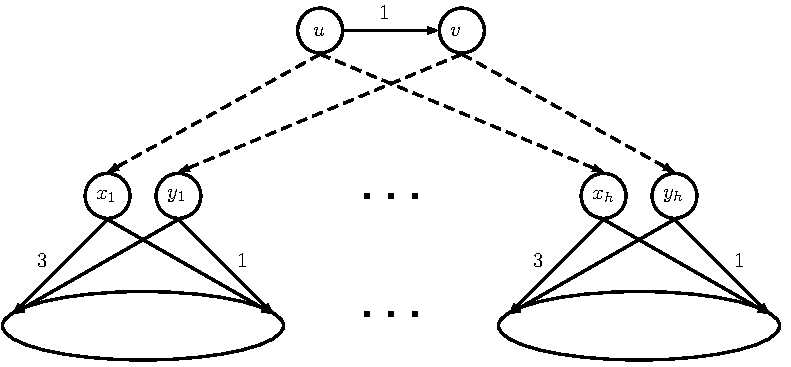
\includegraphics[scale=0.6]{TexImg/Treelike.pdf}
\end{figure}

The general case works in the same fashion.
We make the sparsity grow to $h^k$ by creating two complete, $k$-level, $h$-ary trees $T$ and $T'$.
Connect the root of $T$ to the root of $T'$ and the leafs of both trees are shared.
Observe that the number of nodes is 
\begin{align*}
n &=[\text{$k$-level $h$-ary tree}] + [\text{$(k-1)$-level $h$-ary tree}]\\
&= \frac{h^{k+1}-1}{h-1} + \frac{h^k-1}{h-1},
\end{align*}
therefore the sparsity is $\Theta(n)$, the worst possible.
\end{proof}

It is conjectured that road networks have small HD.
Is there evidence to conjecture small CHD in these networks?
We show how doubling dimension plus an additional property, defined bellow, do imply a positive answer.
A network is said to have doubling dimension $\alpha$ if, for any $r>0$, every ball of radius $2r$ can be covered by at most $\alpha$ balls of radius $r$ \anote{A tad vague because of forward and backward balls, I didn't find references with doubling dimension and directed graphs}.
A path $P'$ \emph{partially witnesses} $P$ if $P'\subseteq P$ and $P'$ is ``long enough''.
Formally, we define the following relation for path systems.

\begin{definition}
Let $\beta\geq 1$.
We say that a path system $\calQ'$ is a $\beta$-witness of the path system $\calQ$ if, for every $Q\in\calQ$, exists $Q'\in\calQ'$ such that $Q'\subseteq Q$ and $\ell(Q')\geq \frac{1}{\beta}\ell(Q)$.
\end{definition}

We explore first when the system of shortest paths $\calP$ is a partial witness for the system of efficient paths $\PE$.
At an intuitive level, the partial witness property says that efficient and shortest paths are not completely different, i.e., if $Q$ is efficient, some fraction of $Q$ is shortest.
As a consequence, an important node hitting numerous paths in $\calP$, should also hit many paths in $\PE$.
The bad examples in Proposition~\ref{prop:treelike} exploit networks that do not have partial witnesses.
We stress that doubling dimension depends only on $G$ and $\ell$; the partial witness property depends on the interplay between $G$, $c$ and $\ell$.

\begin{proposition}\label{prop:doubling}
Assume $G$ is $\alpha$-doubling and $\calP$ is a $\beta$-witness for $\PE$.
If $(G,\ell)$ admits an $(h,r)$-SPHS for any $r$, then $(G,\ell,c)$ admits an $(\alpha^{\ceil{\log_2\beta}} h,r)$-EPHS for any $r$.
\end{proposition}
\begin{proof}
Let $r>0$, we need to construct a hitting set $C^E$ for $\calP_r^E$.
Define $k:=\ceil{\log_2\beta}$ and observe that $\frac{1}{\beta}\geq 2^{-k}$.
Take $C$ as the hitting set for $\calP_{2^{-k}r}$, which is guaranteed to be sparse with respect to balls of radius $2^{-k+1}r$.
Define the desired set by
\[
C^E:=\{v\in C: v \text{ is in some $r$-efficient path} \}.
\]

Since $\calP$ is a $2^{-k}$-witness for $\PE$, $C^E$ is indeed a hitting set for $\PE_r$.
We are only left to prove the sparsity.
Take some $u\in V$, by doubling dimension we can cover $\Bf_{2r}(u)$ by at most $\alpha^k$ balls of radius $2^{-k+1}r$.
Each of these balls contains at most $h$ elements of $C$, therefore the sparsity is as claimed.
The argument for backward balls is identical.
\end{proof}

\begin{remark}
The existence of a $\beta$-witness is not enough to bound the CHD.
Nevertheless, as discussed in Section~\ref{sec:multi_scale}, the existence of $(h,r)$-SPHS already allows the construction of HL.
\end{remark}